%\section{Proton Recoil Detector}


\section{Improvment to Projection of new Measurement}
\begin{figure}[!ht]
 \begin{center}
    \subfloat[w/o PRD]{
      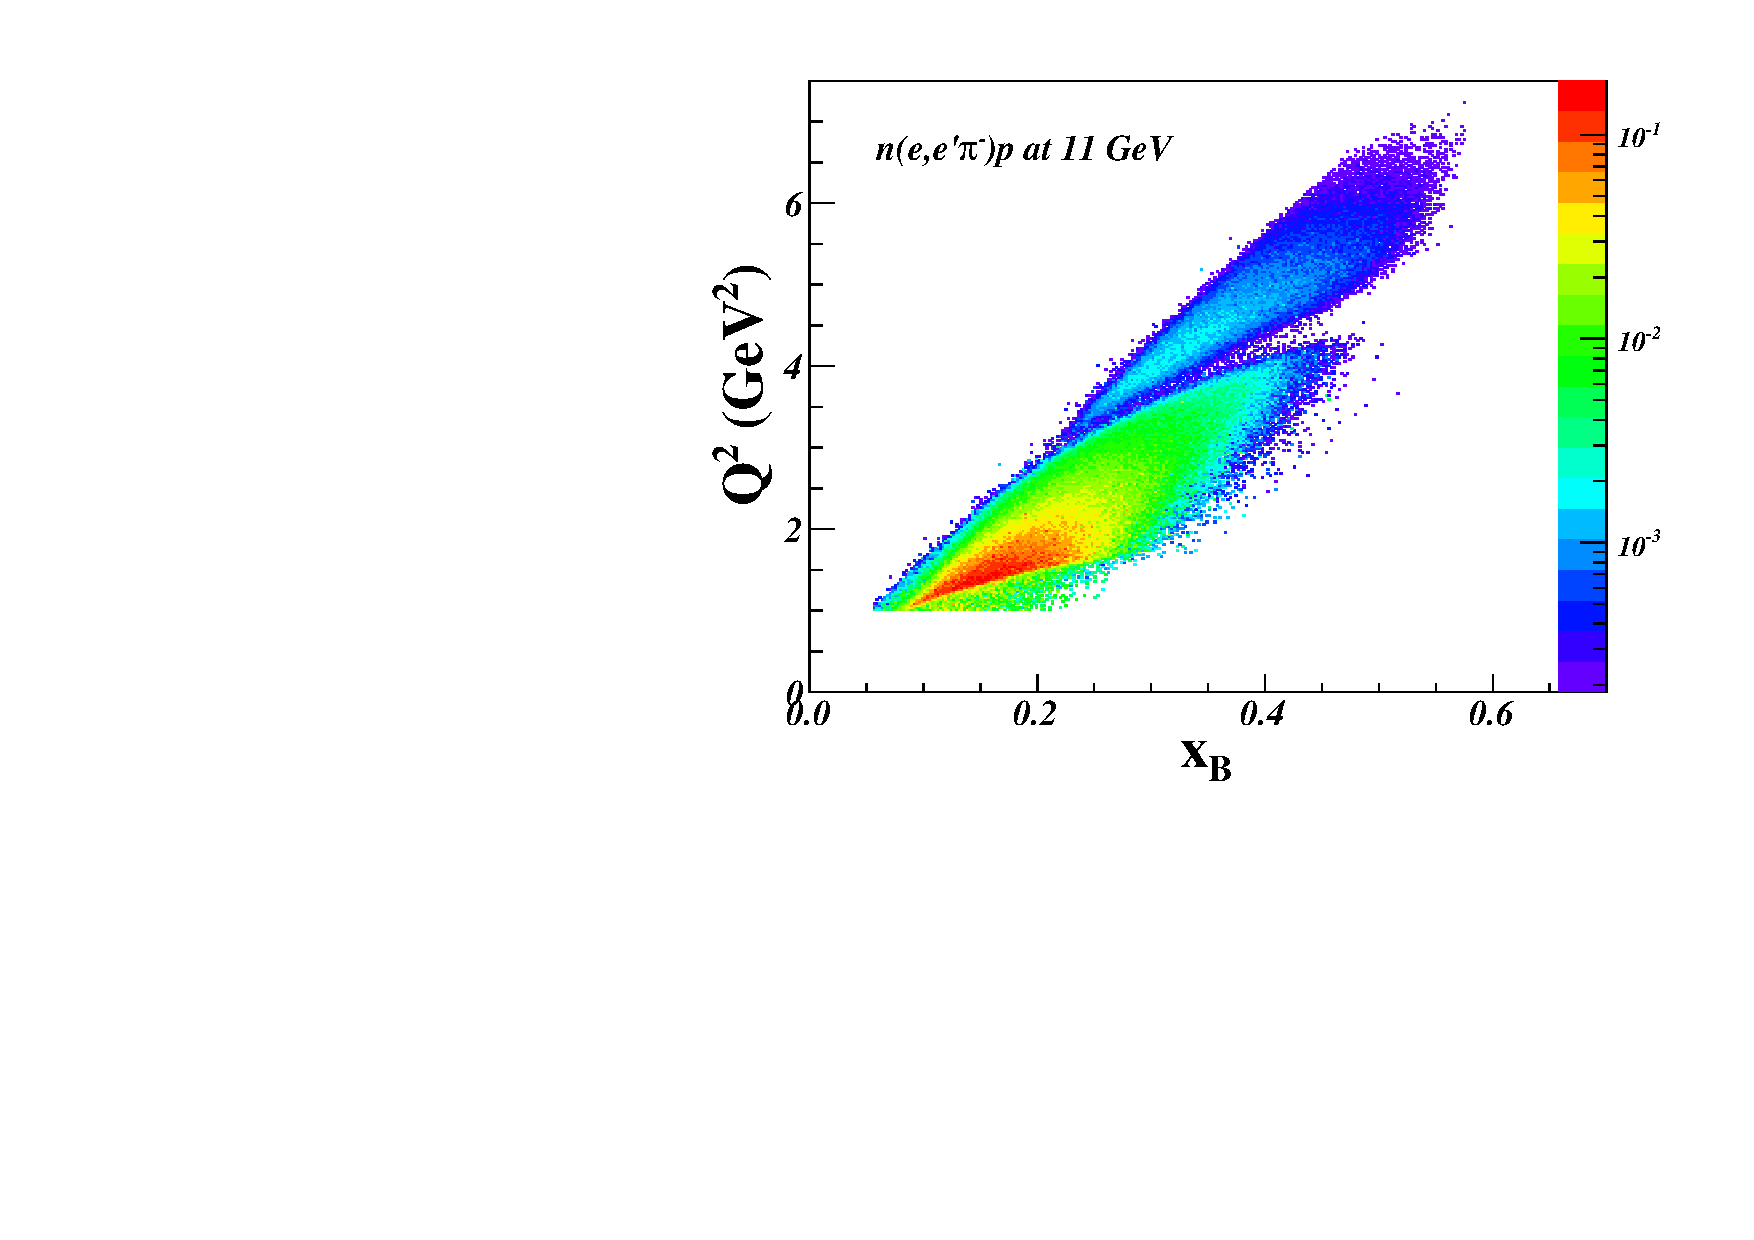
\includegraphics[type=pdf,
        ext=.pdf,read=.pdf,width=0.45\textwidth]{./figures/E11_Q2_x_fermi}
         }
           \subfloat[w/ PRD]{
      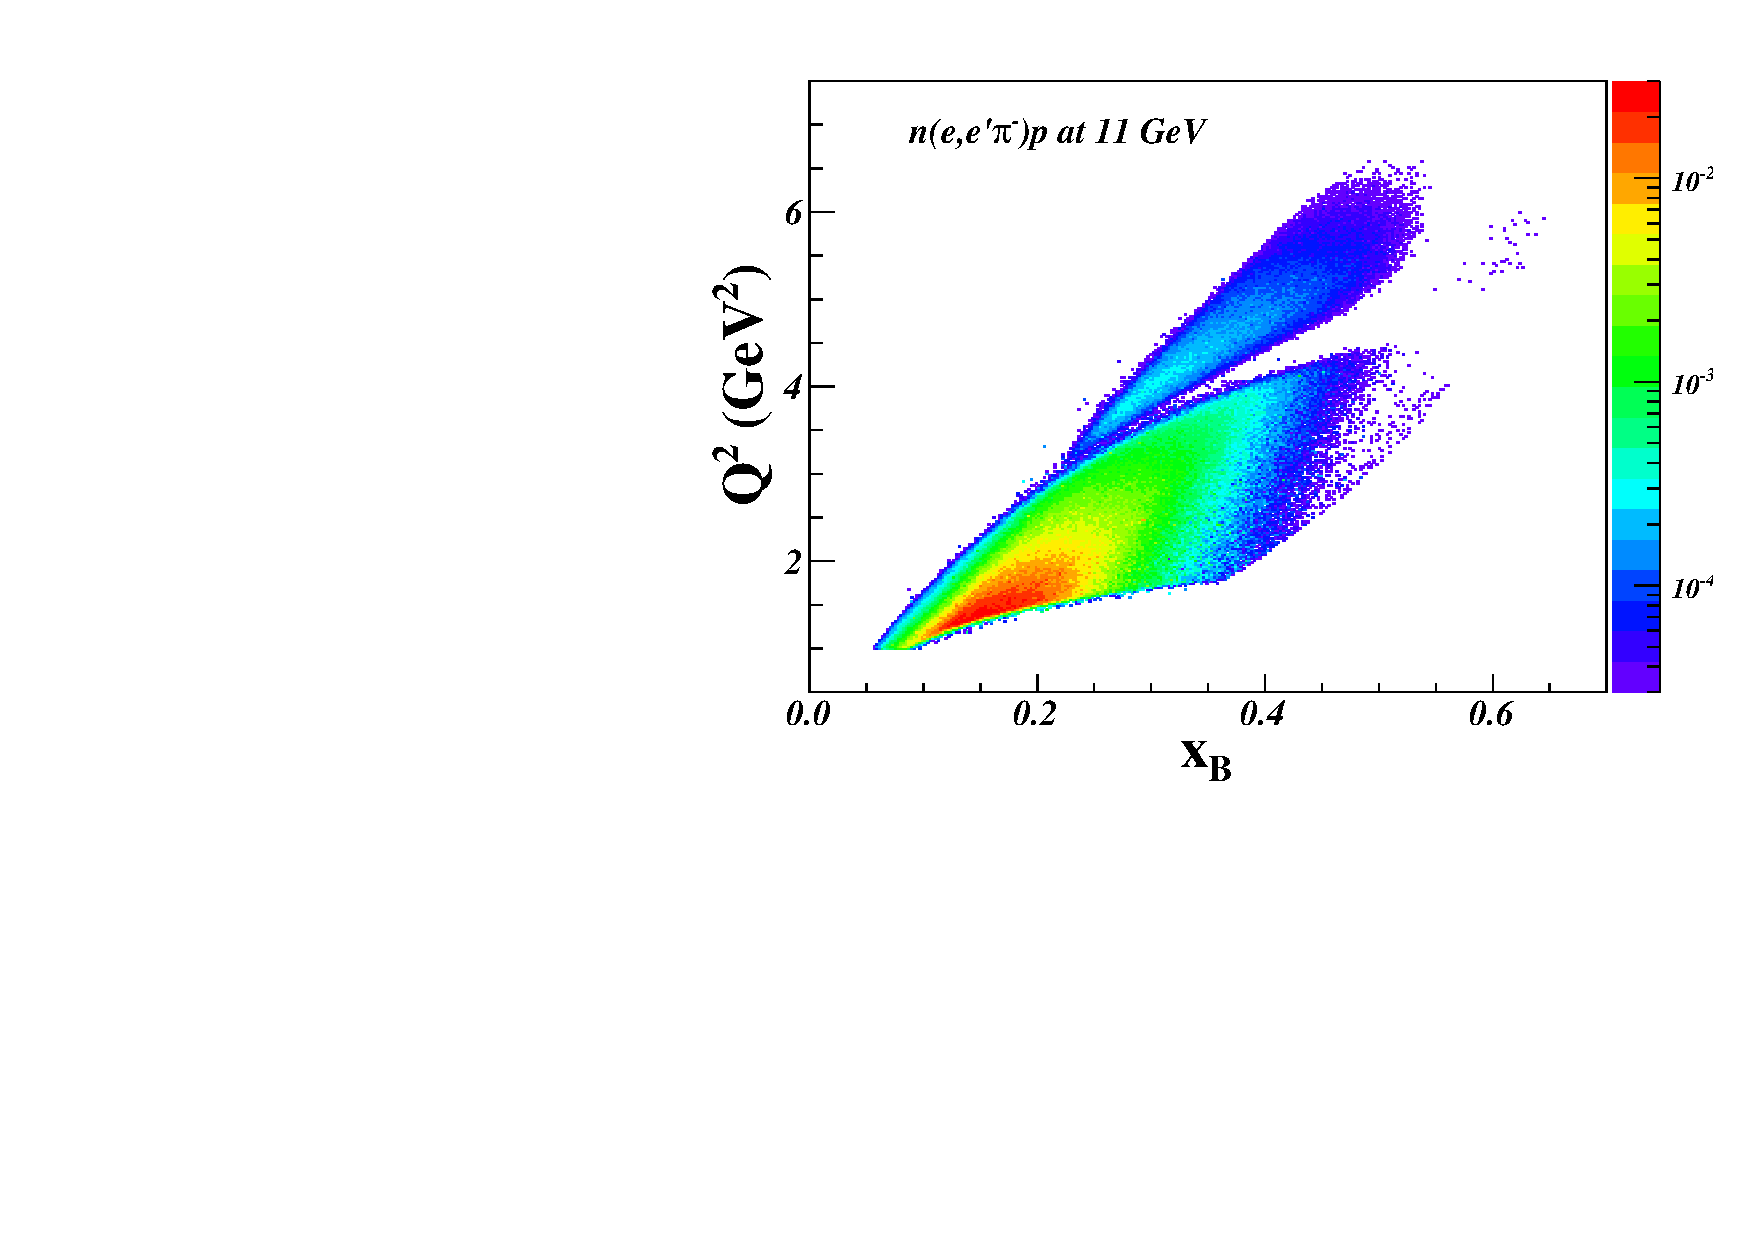
\includegraphics[type=pdf,
        ext=.pdf,read=.pdf,width=0.45\textwidth]{./figures/E11_Q2_x_prd_fermi}
           }
 \caption[The kinematic coverage at different acceptances.]{\footnotesize{The
     kinematic coverage at different acceptances at 11~GeV, when detecting all
recoil protons w/o (left) or w/ (right) an additional proton detector. Colors correspond to rates
(Hz) in log scale.}}
  \label{kin_cor_prd}
  \end{center}
\end{figure}
The kinematic coverage in $Q^{2}$ vs. $x_{B}$ is shown in Fig.~\ref{kin_cor_prd},
when adding a new proton recoil detector to detect the rest of the recoil
protons at larger angle ($24^{\circ}\sim50^{\circ}$), in addition to the existing SoLID detectors which cover the angle from  $8^{\circ}$ to $24^{\circ}$.


\begin{figure}[!ht]
 \begin{center}
     \subfloat[w/o PRD]{
	       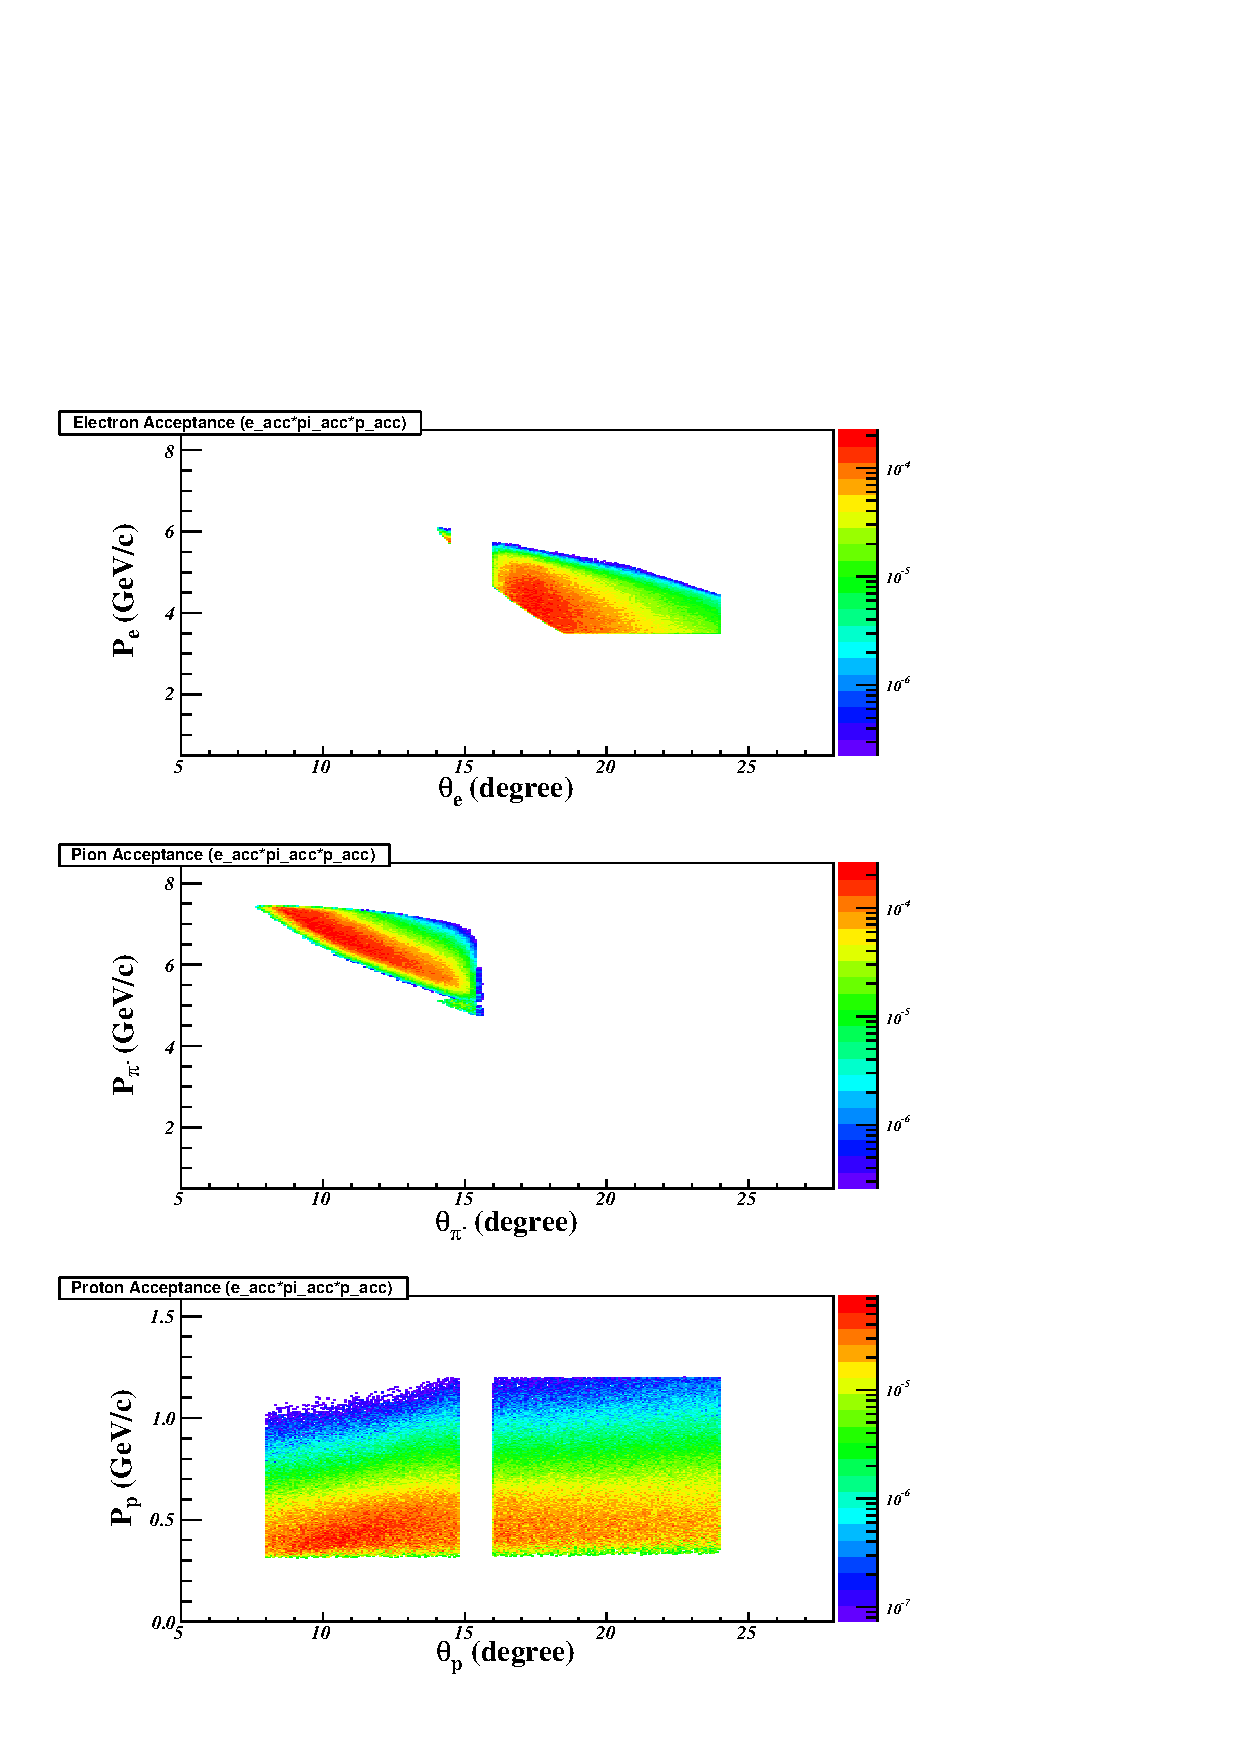
\includegraphics[type=pdf,
     ext=.pdf,read=.pdf,width=0.45\textwidth]{./figures/E11_acc_epip_Q2gt4}}
     \subfloat[w/ PRD]{
     ext=.pdf,read=.pdf,width=0.45\textwidth]{./figures/E11_acc_epi_Q2gt4}}
	 
  \caption[The acceptance of the momenta and scattering angles for electrons,
    $\pi^{-}$ and protons]{\footnotesize{The acceptance of the momenta and
    polar angles w/o (left) or w/ (right) the PRD. In each panel, he top, middle and
    bottom plots are for electrons, $\pi^{-}$ and protons, respectively. A
    cut of $Q^{2}>4~\mathrm{GeV^{2}}$ is applied. Colors correspond to rates
    (Hz) in log scale.}}
  \label{p_theta_prd}
  \end{center}
\end{figure}


\begin{table}[!ht]
\centering
\begin{tabular}{|c|c|c|}
 \hline
  1$<Q^2<$4~GeV$^2$ & $Q^2>$4~GeV$^2$ & Total\\
 \hline
\multicolumn{3}{|c|}{DEMP: $\vec{n}(e,e'\pi^{-}p)$ Triple-Coincidence (Hz)}\\
 \hline
 25.59 (6.11)   &  0.54 (0.26) & 26.13 (6.37)   \\
 \hline
\multicolumn{3}{|c|}{SIDIS: $\vec{n}(e,e'\pi^{-})X$ Double-Coincidence (Hz)}\\
 \hline
        1388.85 & 35.77        & 1424.62   \\
 \hline
\end{tabular}
\caption[Triple-Coincidence rates for
  neutron-DEMP]{\footnotesize{Triple-Coincidence rates for DEMP events compared
    with the SIDIS rates. Numbers in brackets are the DEMP rates with only
    detecting protons using only the SoLID detectors. The online production
    trigger will be the SIDIS double-coincidence trigger of which rates are
    also given.}}
\label{rate_table_prd}
\end{table} 



\begin{figure}[!ht]
 \begin{center}
       \subfloat[w/o PRD]{
      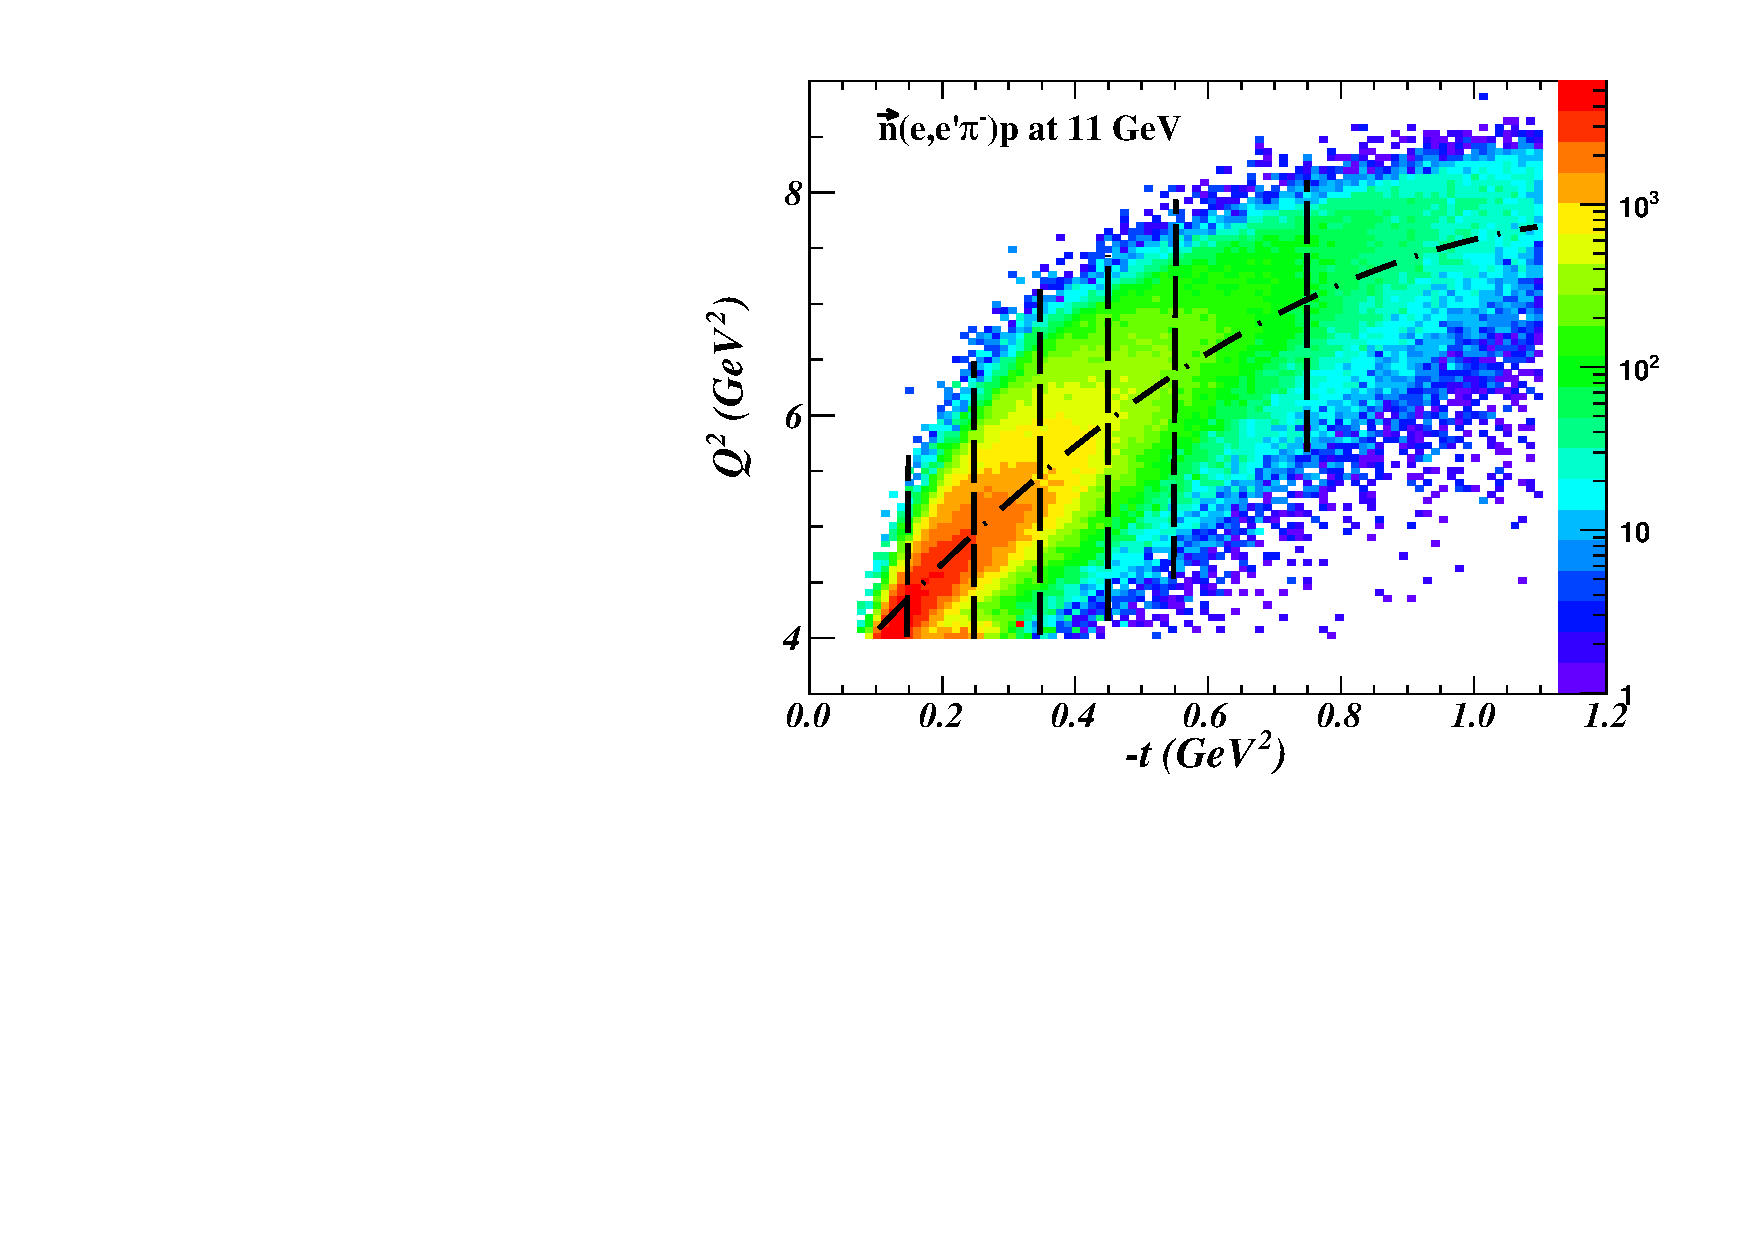
\includegraphics[type=pdf,
        ext=.pdf,read=.pdf,width=0.5\textwidth]{./figures/E11_Q2_t_bin_Fermi} }
        \subfloat[w/ PRD]{
      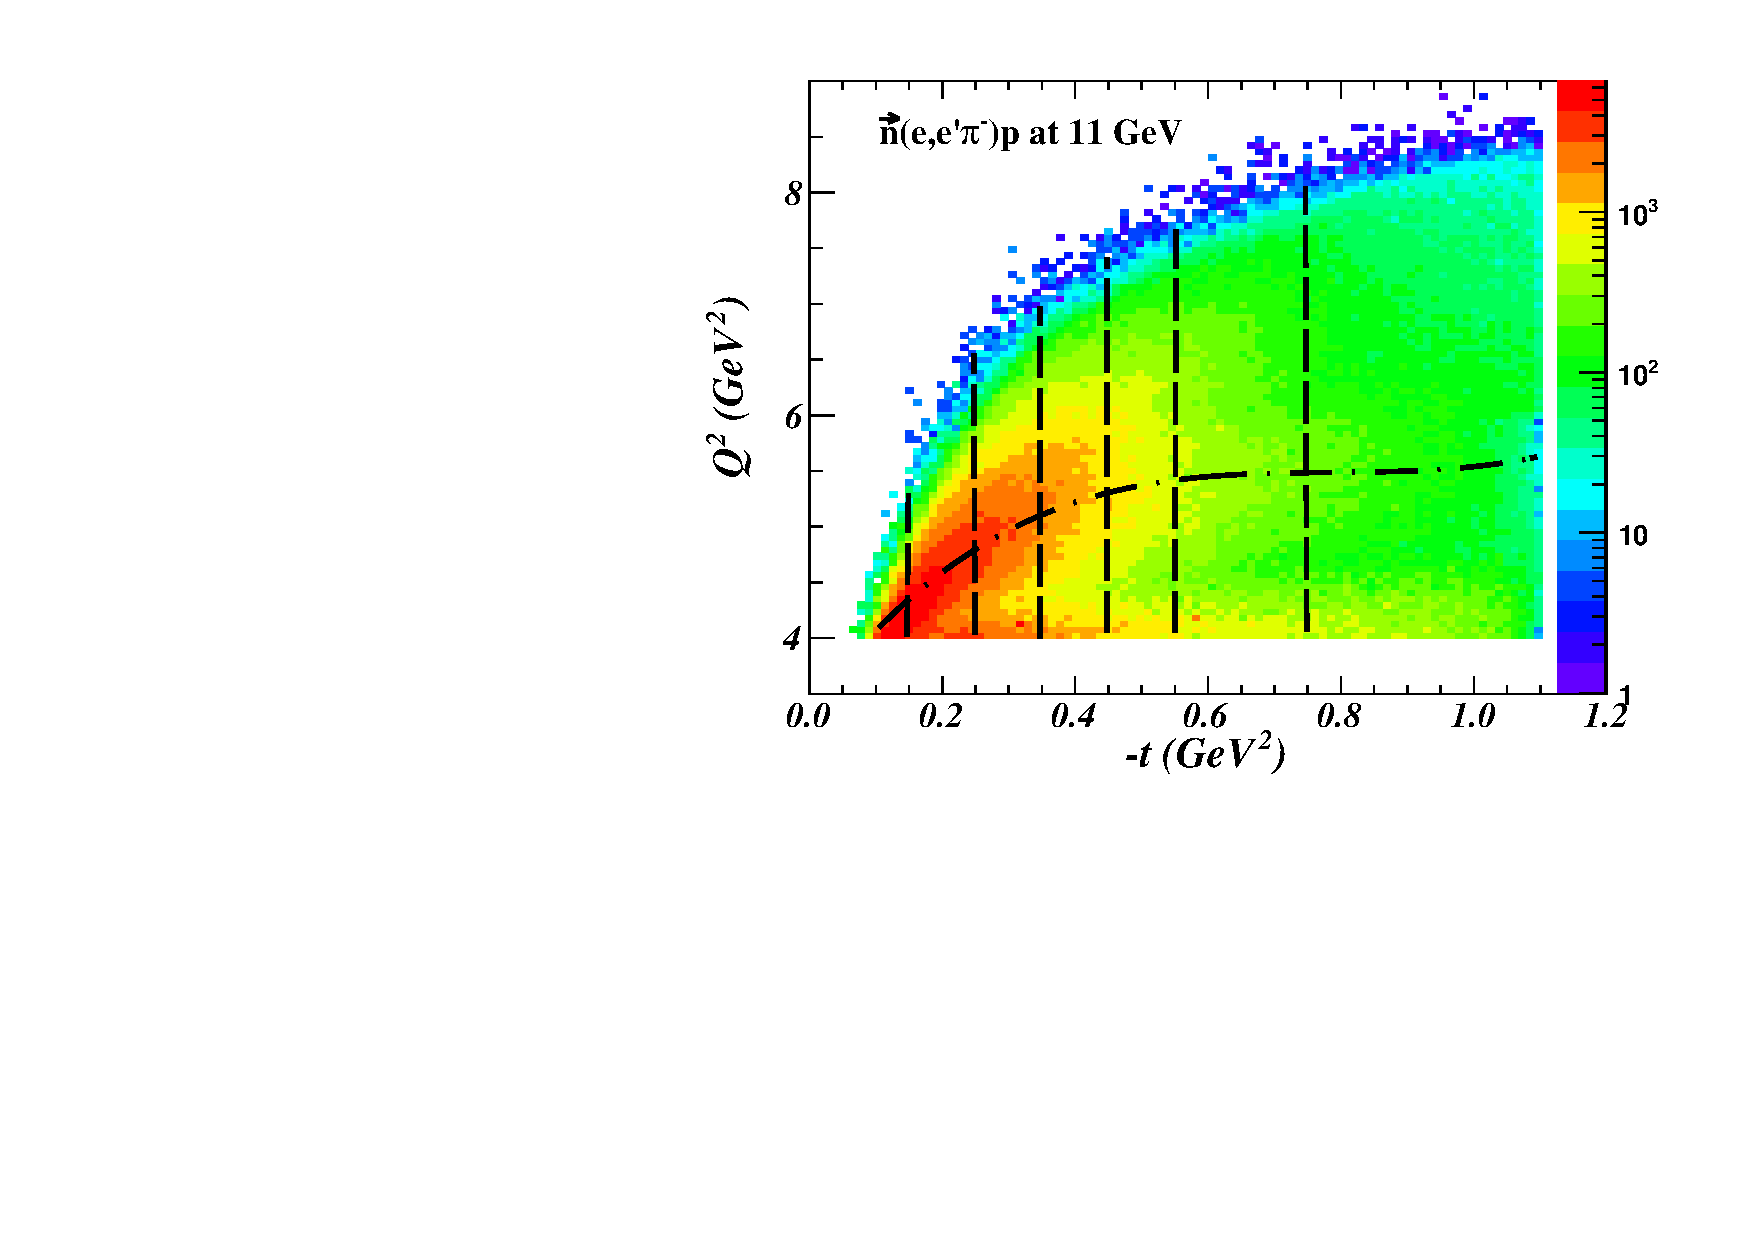
\includegraphics[type=pdf,
        ext=.pdf,read=.pdf,width=0.5\textwidth]{./figures/E11_Q2_t_bin_prd_Fermi} }
   \caption[$Q^{2}$ vs. $-t$]{\footnotesize{$Q^{2}$ vs. $-t$ where the black
dash lines specify the boundaries of 7 $-t$ bins and the black dash-dot lines
indicate the additional two $Q^{2}$ bins.  The color panel indicates the raw
counts with 48 days of beam time at 11~GeV.}}
  \label{Q2_t_bin_prd}
  \end{center}
\end{figure}

\begin{figure}[!ht]
 \begin{center}
         \subfloat[w/o PRD]{
               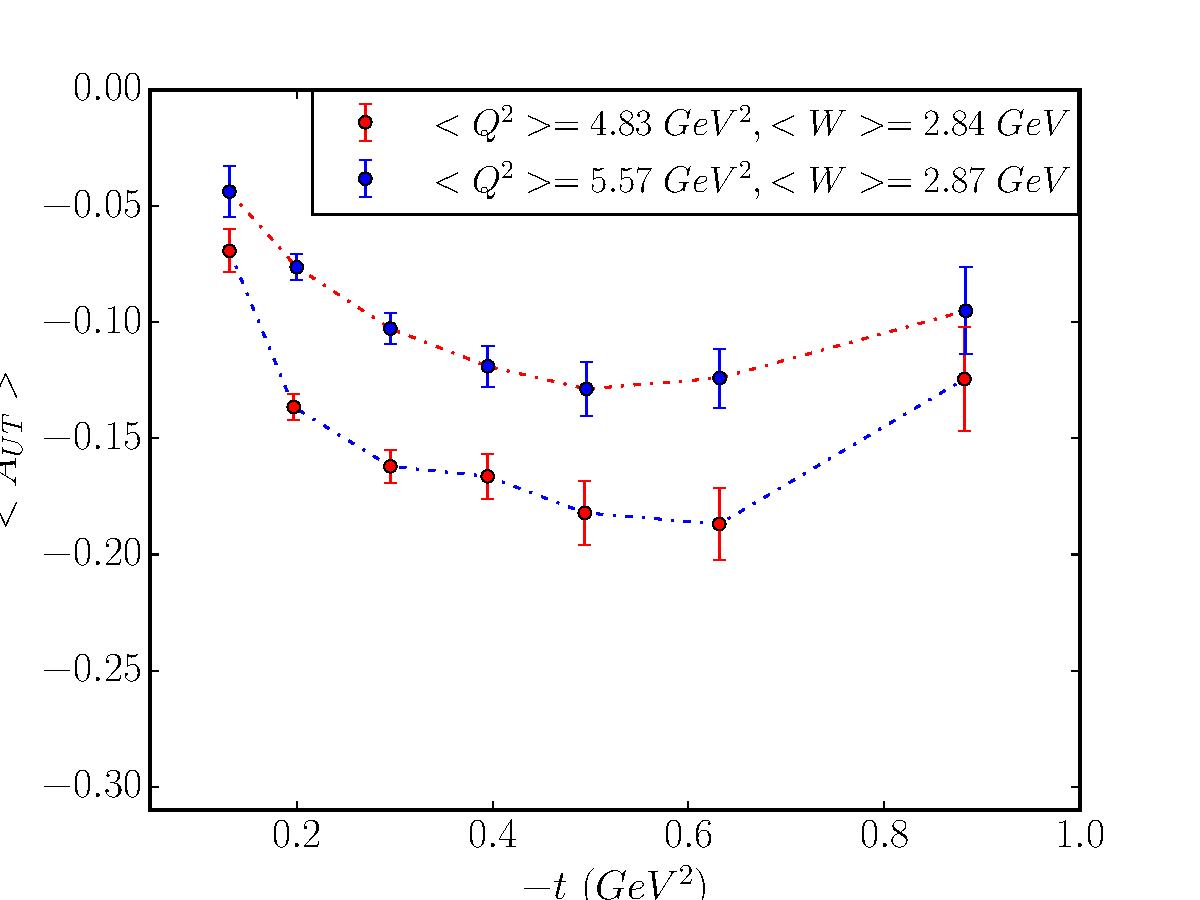
\includegraphics[type=pdf,
        ext=.pdf,read=.pdf,width=0.45\textwidth]{./figures/bin_asym_t_fermi} }
            \subfloat[w/ PRD]{
      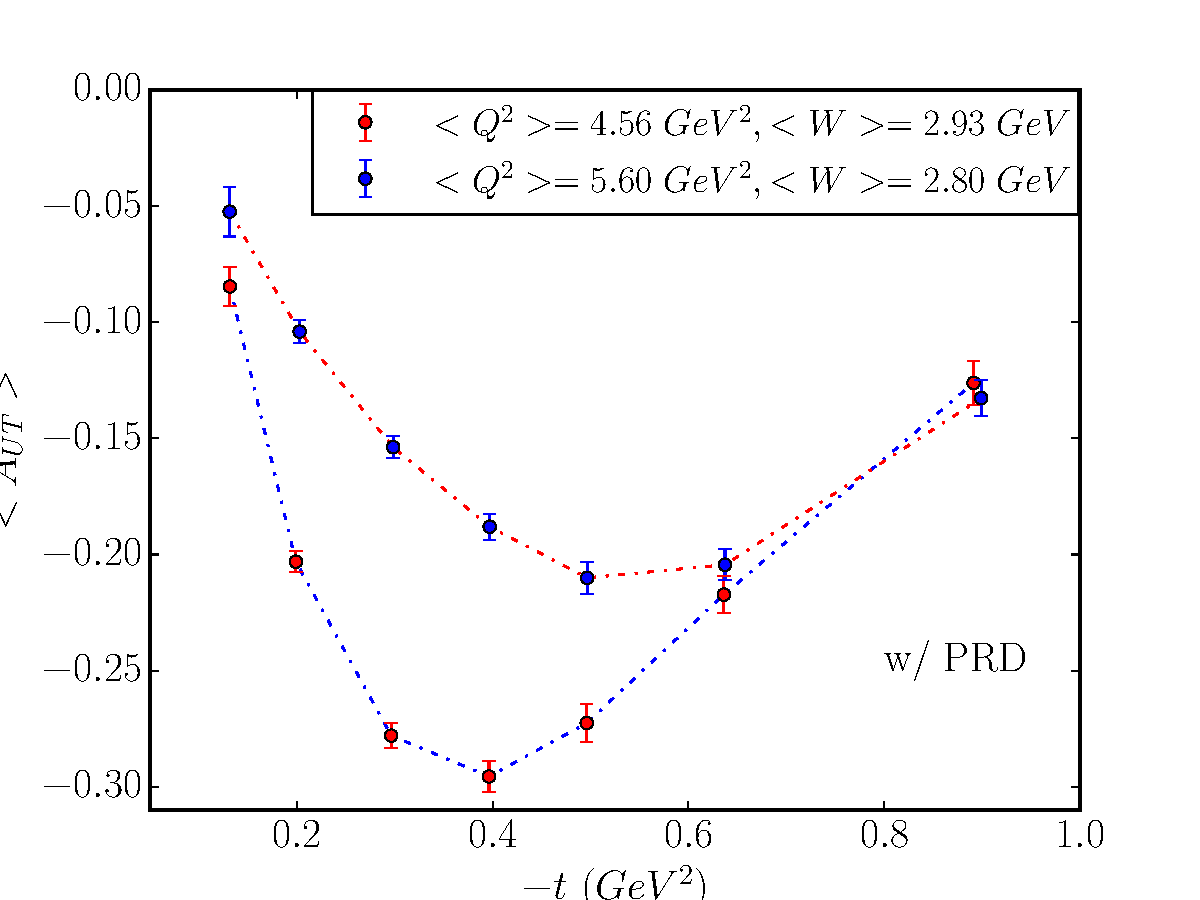
\includegraphics[type=pdf,
        ext=.pdf,read=.pdf,width=0.45\textwidth]{./figures/bin_asym_t_prd_fermi} }
      \caption{\footnotesize{Projection of target single spin asymmetry
          ($A_{UT}$) as a function of $-t$ for DEMP with transversely polarized
          $\mathrm{^{3}He}$ at $E_{0}$=11~GeV (directly compare with
Fig.~\ref{fig:hermes_aut}).  The data in each $-t$ bin are further divided into
two $Q^{2}$ bins with similar statistics.  The error bars are the projected
statistical uncertainties defined in Eq.~\ref{stat_err}. The asymmetry value in
each bin is predicted with the model given in Appendix-A and is diluted due to
not separating the L/T contributions. The left plot shows the projection w/o a
new proton recoil detector, while the right plot shows a better projected
result with a new detector in addition. One can see the average asymmetries are
also changed between two configurations because the asymmetry dilution
strongly depends on $Q^{2}$, which changes w/ or w/o the PRD.}}
  \label{asym_t}
  \end{center}
\end{figure}


\begin{table}[!ht]
\centering
 \small
\begin{tabular}{|c|c|c|c|c|c|c|c|}
\multicolumn{8}{c}{ (a) w/o PRD} \\
\hline
       &  t-bin\#1 & t-bin\#2 & t-bin\#3 & t-bin\#4 & t-bin\#5 & t-bin\#6 & t-bin\#7 \\
\hline $<-t>$ &  0.13 &  0.20 & 0.30 & 0.39 & 0.49 & 0.63 & 0.88 \\
\hline
\multicolumn{8}{|c|}{$Q^{2}$ bin-set\#1 } \\
\hline
$<Q^{2}>$      &  4.13 &  4.42 & 4.90 & 5.35 & 5.76 & 6.23 & 6.86 \\
$<\sigma_{L}/\sigma_{T}>$   &  6.43 &  5.13 & 3.90 & 3.09 & 2.43 & 1.65 & 0.69 \\
$<f_{L/T}>$    &  0.80 &  0.77 & 0.73 & 0.68 & 0.62 & 0.52 & 0.30 \\
$<A_{UT}>$     &  -6.93$\times 10^{-2}$ &  -1.36$\times 10^{-1}$ & -1.62$\times 10^{-1}$ &
 -1.66$\times 10^{-1}$ & -1.82$\times 10^{-1}$ & -1.87$\times 10^{-1}$ & -1.24$\times 10^{-1}$ \\               
$\delta A_{UT}$&  9.23$\times 10^{-3}$ &  5.62$\times 10^{-3}$ & 7.16$\times 10^{-3}$ & 
9.72$\times 10^{-3}$ & 1.39$\times 10^{-2}$ & 1.54$\times 10^{-2}$ &  2.24$\times 10^{-2}$ \\
$N$           &  3.26$\times 10^{4}$ &  8.73$\times 10^{4}$ & 5.37$\times 10^{4}$ 
& 2.91$\times 10^{4}$ & 1.42$\times 10^{4}$ & 1.15$\times 10^{4}$ & 5.50$\times 10^{3}$ \\
\hline
\multicolumn{8}{|c|}{$Q^{2}$ bin-set\#2 } \\
\hline 
$<Q^{2}>$     &  4.39 &  4.93 & 5.58 & 6.13 & 6.59 & 7.09 & 7.73 \\
$<\sigma_{L}/\sigma_{T}>$&  7.19 &  6.38 & 5.51 & 4.63 & 3.70 & 2.57 & 1.21 \\
$<f_{L/T}>$   &  0.81 &  0.80 & 0.78 & 0.74 & 0.70 & 0.61 & 0.42 \\
$<A_{UT}>$    &  -4.38$\times 10^{-2}$ &  -7.63$\times 10^{-2}$ & -1.03$\times 10^{-1}$ & 
-1.19$\times 10^{-1}$ & -1.29$\times 10^{-1}$ & -1.24$\times 10^{-1}$ & -9.51$\times 10^{-2}$ \\
$\delta A_{UT}$&  1.13$\times 10^{-2}$ &  5.82$\times 10^{-3}$ & 6.83$\times 10^{-3}$ 
& 9.05$\times 10^{-3}$ & 1.21$\times 10^{-2}$ & 1.32$\times 10^{-2}$ & 1.94$\times 10^{-2}$ \\
$N$          &  2.17$\times 10^{4}$ &  8.19$\times 10^{4}$ & 5.94$\times 10^{4}$ &
  3.38$\times 10^{4}$ & 1.88$\times 10^{4}$ & 1.59$\times 10^{4}$ & 7.32$\times 10^{3}$ \\
\hline
\multicolumn{8}{c}{} \\
\multicolumn{8}{c}{ (b) w/ PRD} \\
\hline
	     &  t-bin\#1 & t-bin\#2 & t-bin\#3 & t-bin\#4 & t-bin\#5 & t-bin\#6 & t-bin\#7 \\
\hline 
$<-t>$       &  0.13 & 0.20   & 0.30   & 0.40   & 0.50   & 0.64   & 0.90  \\
\hline
\multicolumn{8}{|c|}{$Q^{2}$ bin-set\#1 } \\
\hline
$<Q^{2}>$   &  4.12 &  4.34 & 4.59 & 4.74 & 4.83 & 4.86 & 4.84 \\
$<\sigma_{L}/\sigma_{T}>$&  6.41 &  4.90 & 3.37 & 2.32 & 1.62 & 1.02 & 0.46 \\
$<f_{L/T}>$   &  0.80 &  0.76 & 0.69 & 0.60 & 0.52 & 0.40 & 0.23 \\
$<A_{UT}>$ &  -8.46$\times 10^{-2}$ &  -2.03$\times 10^{-1}$ & -2.78$\times 10^{-1}$ & 
-2.96$\times 10^{-1}$ & -2.73$\times 10^{-1}$ & -2.17$\times 10^{-1}$ & -1.26$\times 10^{-1}$ \\
$\delta A_{UT}$&  8.57$\times 10^{-3}$ &  4.58$\times 10^{-3}$ & 5.30$\times 10^{-3}$ & 
6.58$\times 10^{-3}$ & 8.24$\times 10^{-3}$ & 7.97$\times 10^{-3}$ & 9.57$\times 10^{-3}$ \\
$N$     &  3.77$\times 10^{4}$ &  1.31$\times 10^{5}$ & 9.61$\times 10^{4}$ &
6.22$\times 10^{4}$ & 3.98$\times 10^{4}$ & 4.30$\times 10^{4}$ & 3.02$\times 10^{4}$ \\   
\hline
\multicolumn{8}{|c|}{$Q^{2}$ bin-set\#2 } \\
\hline 
$<Q^{2}>$   &  4.40 &  4.88 & 5.39 & 5.77 & 6.07 & 6.35 & 6.66 \\
$<\sigma_{L}/\sigma_{T}>$   &  7.19 &  6.15 & 4.96 & 3.84 & 2.88 & 1.81 & 0.69 \\
$<f_{L/T}>$  &  0.81 &  0.79 & 0.76 & 0.71 & 0.65 & 0.53 & 0.30 \\
$<A_{UT}>$   &  -5.24$\times 10^{-2}$ &  -1.04$\times 10^{-1}$ & -1.54$\times 10^{-1}$ 
& -1.88$\times 10^{-1}$ & -2.10$\times 10^{-1}$ & -2.04$\times 10^{-1}$ & -1.33$\times 10^{-1}$ \\
$\delta A_{UT}$&  1.07$\times 10^{-2}$ &  4.86$\times 10^{-3}$ & 4.86$\times 10^{-3}$ & 
5.57$\times 10^{-3}$ & 6.88$\times 10^{-3}$ & 6.62$\times 10^{-3}$ & 7.64$\times 10^{-3}$ \\
$N$         &  2.42$\times 10^{4}$ &  1.17$\times 10^{5}$ & 1.17$\times 10^{5}$& 8.85$\times 10^{4}$ 
& 5.78$\times 10^{4}$ & 6.24$\times 10^{4}$ & 4.73$\times 10^{4}$ \\
\hline
\end{tabular}
\caption[Detailed information of projected bins]{\footnotesize{Detailed
information of projected bins from the new DEMP measurements with SoLID, while
$<Q^{2}>$ and $<-t>$ are in the unit of GeV$^{2}$. The top (bottom) table is
with respect to the case of proton detection w/o (w/) a new PRD. The data are
divided into 14 $-t$ bins in both $-t$ (7 bins) and $Q^{2}$ (2 bins).}}
\label{asym_bin_table_prd}
\end{table} 


\section(Improvement to the Missing Mass and Background Rejection)

\begin{figure}[!ht]
\begin{center}
\subfloat[w/o PRD]{
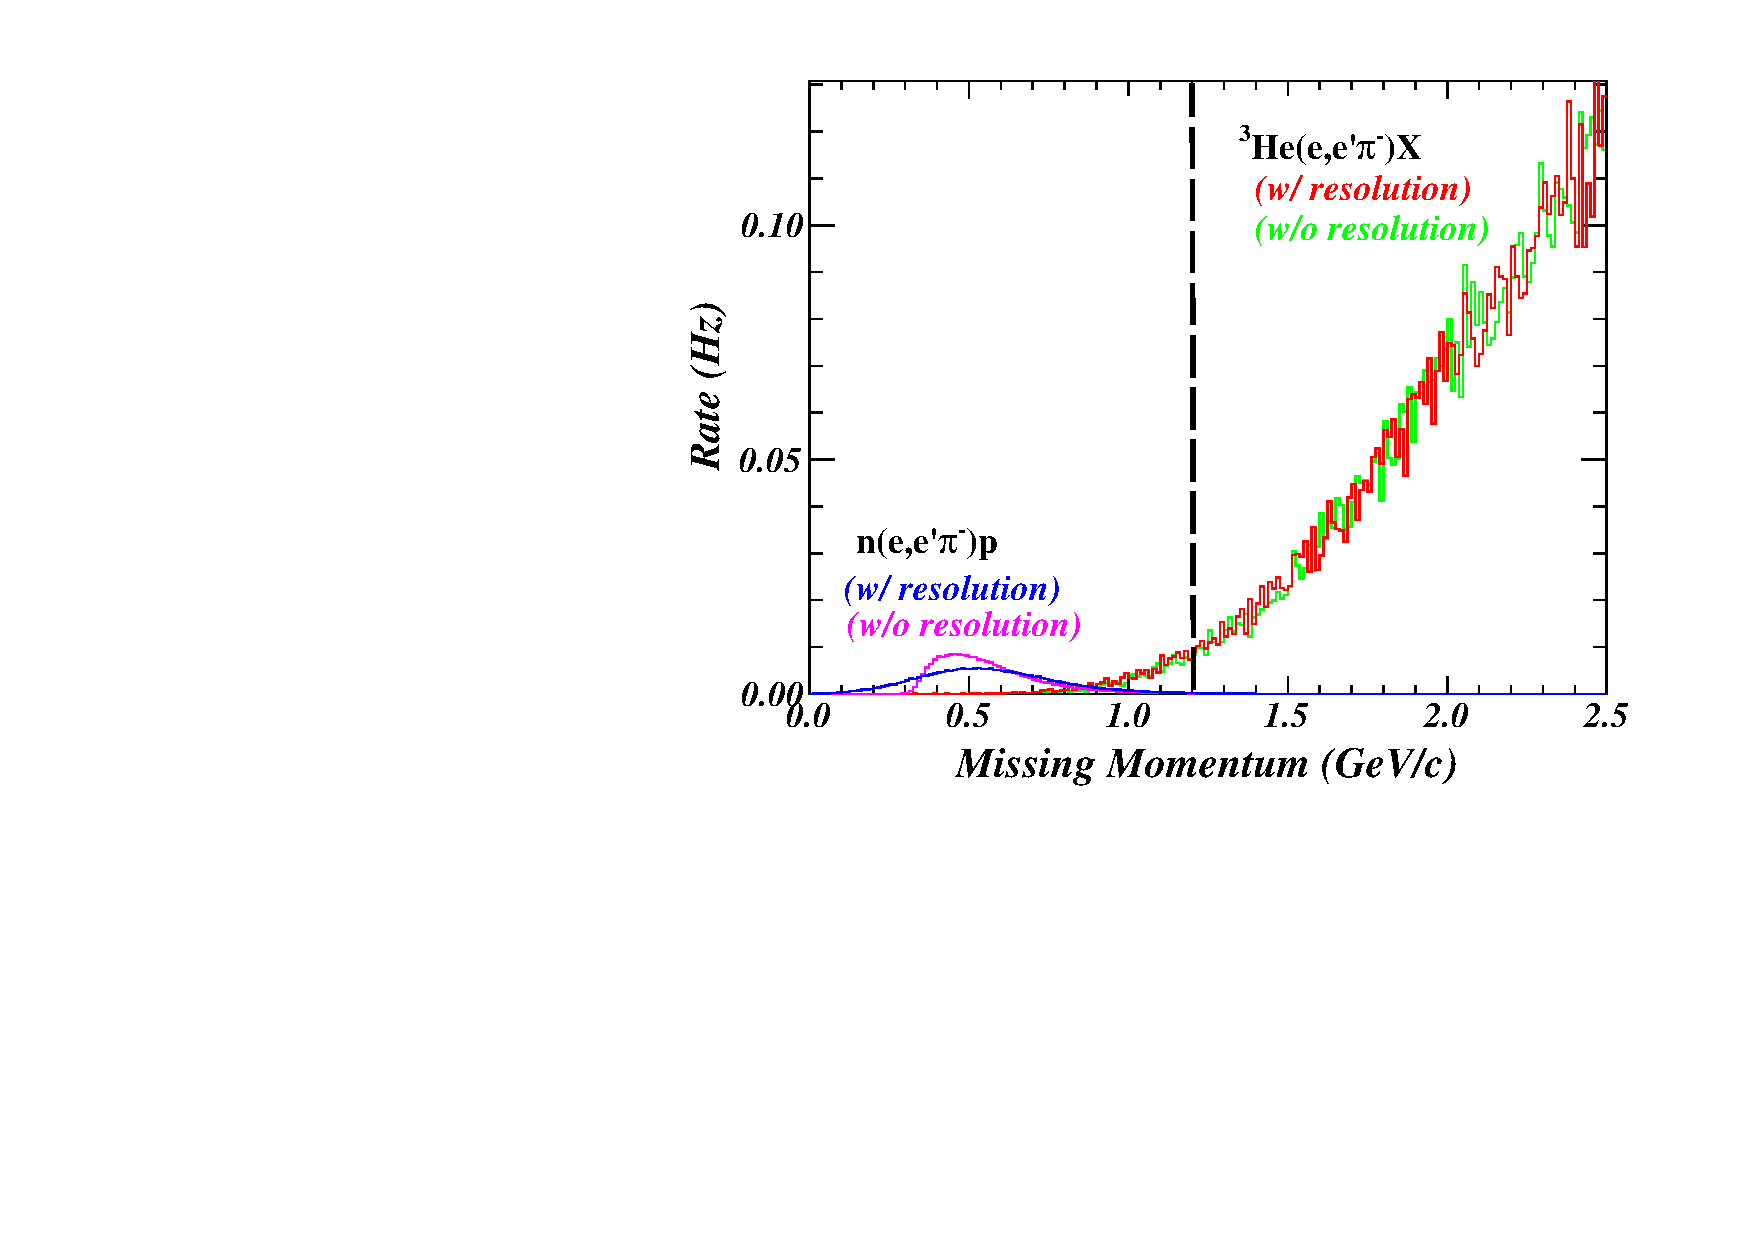
\includegraphics[type=pdf,ext=.pdf,read=.pdf,width=0.5\textwidth]{./figures/Missing_P_Fermi}}
\subfloat[w/ PRD]{
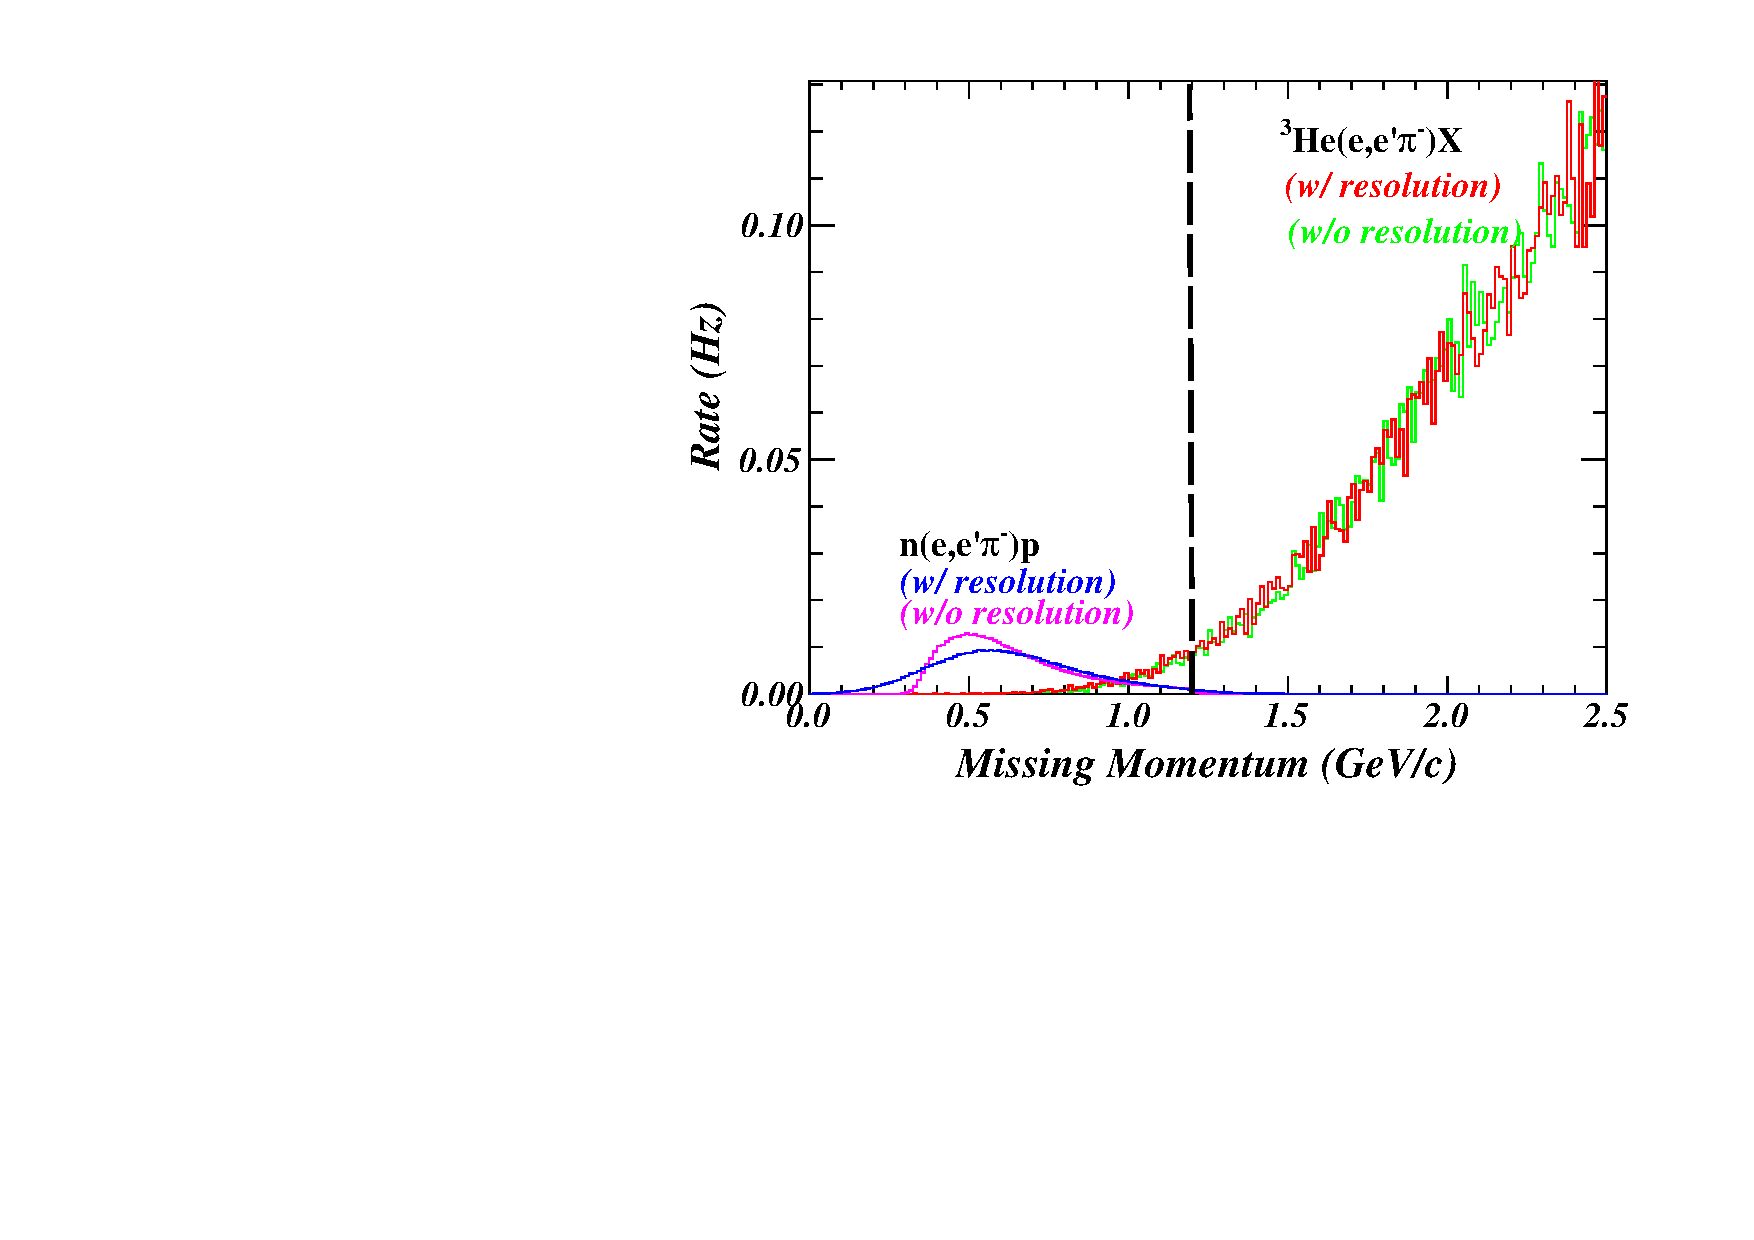
\includegraphics[type=pdf,ext=.pdf,read=.pdf,width=0.5\textwidth]{./figures/Missing_P_PRD_Fermi}} 
\caption[Missing Momentum]{\footnotesize{Missing momentum spectra of DEMP
and SIDIS events. The missing momentum distributions are well separated between
the two processes and one can apply a cut at $P_{miss}<1.2$~GeV/c (indicated by the
black dashed line) to remove most of the SIDIS events.}}
  \label{missing_mom_prd}
  \end{center}
\end{figure}

\begin{figure}[!ht]
 \begin{center}
       \subfloat[w/o PRD]{
      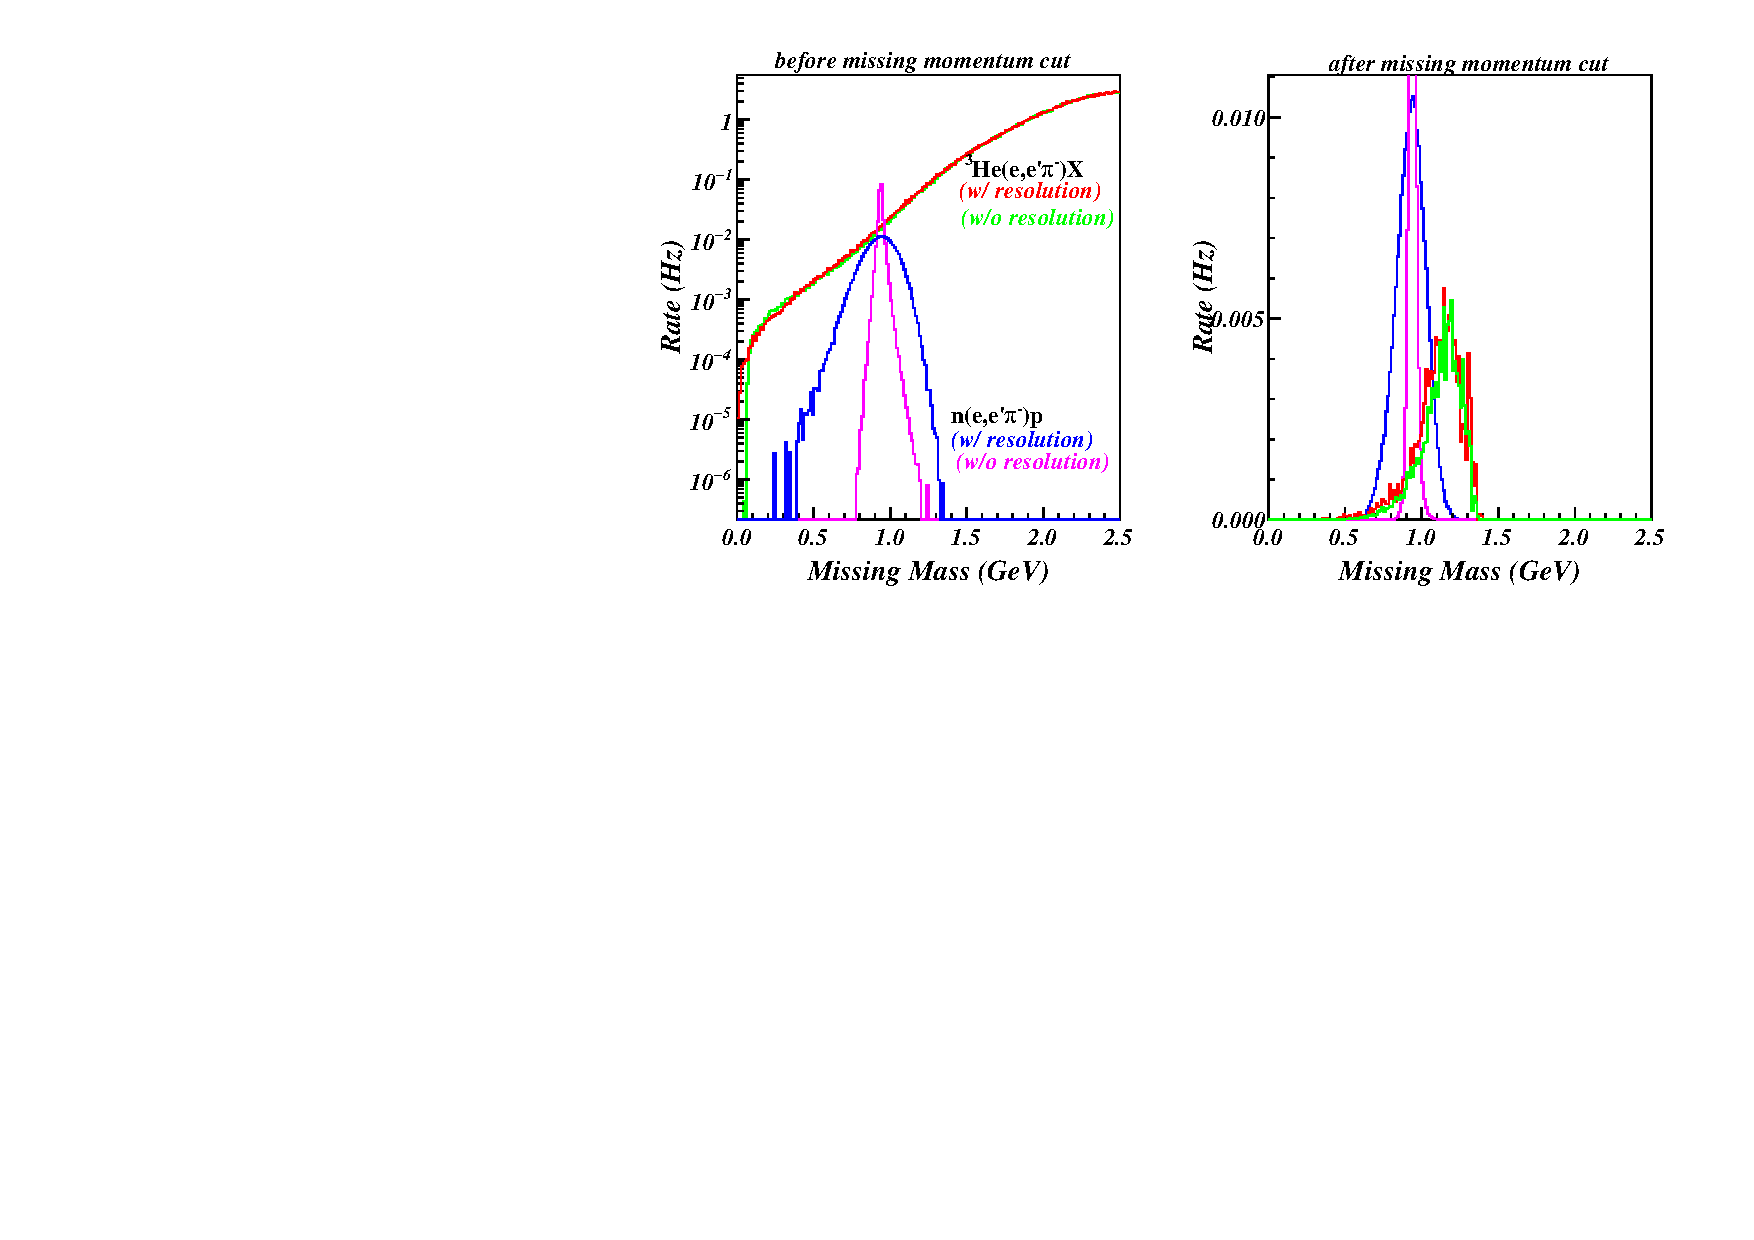
\includegraphics[type=pdf,
        ext=.pdf,read=.pdf,width=0.85\textwidth]{./figures/Missing_Mass_Fermi} }\\
          \subfloat[w/ PRD]{
      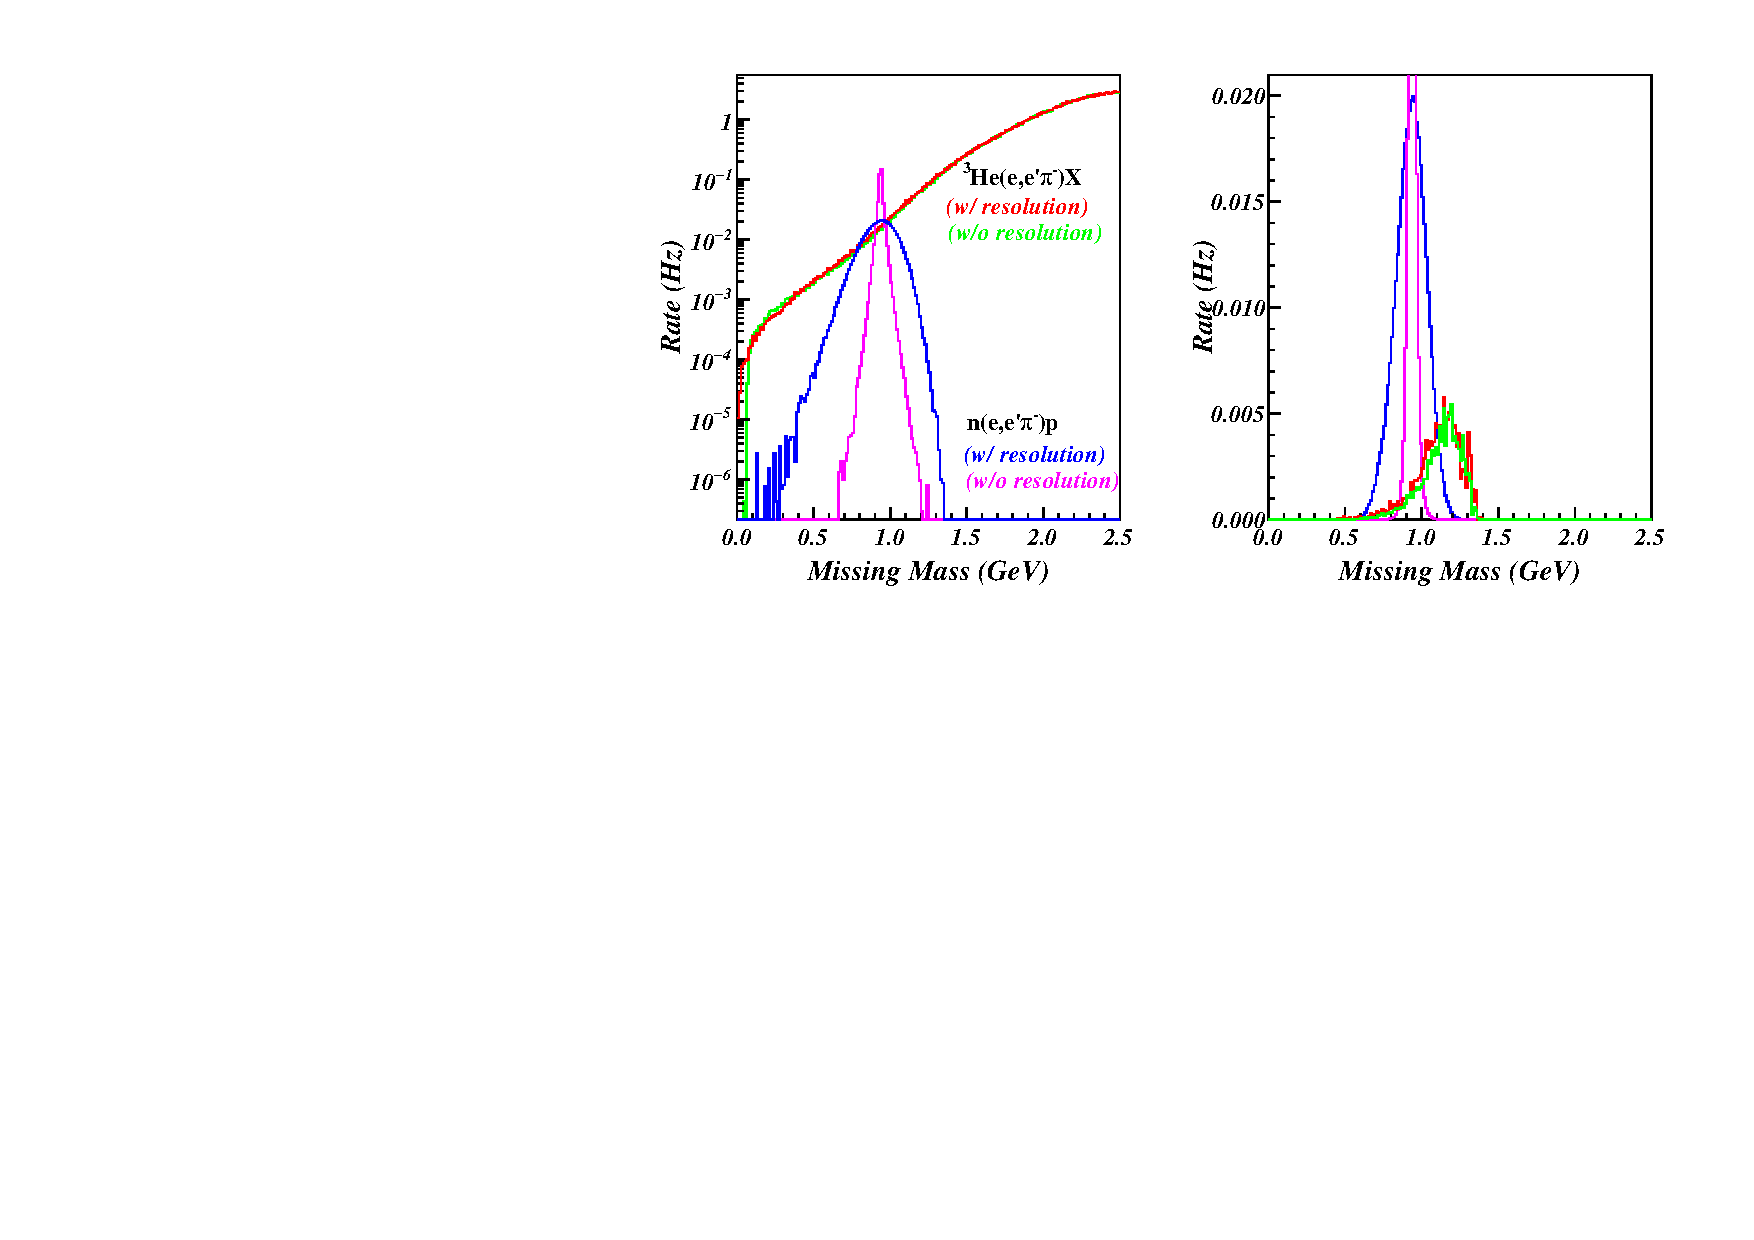
\includegraphics[type=pdf,
        ext=.pdf,read=.pdf,width=0.85\textwidth]{./figures/Missing_Mass_PRD_Fermi} } 
   \caption[Missing Mass]{\footnotesize{Missing mass spectra of DEMP and SIDIS
events. Top (bottom) panel shows the missing mass distribution of DEMP events
w/o (w/) proton detection by a new PRD.  The left (right) plot of each panel 
shows the background contamination from SIDIS events before (after) the
missing momentum cut shown in Fig.~\ref{missing_mom}. The broadening effect of
the missing mass due to only the Fermi motion is indicated by the magenta
curve. The SIDIS background is already small compared with DEMP events before
optimizing the cut. The actual SIDIS background should be much smaller, since
we overestimated the SIDIS rate by assuming all target fragments ("X") in the
SIDIS process contain protons.}}
  \label{missing_mass_prd}
  \end{center}
\end{figure}


\section{Requirements and Conceptual Design}

\begin{figure}[!ht]
 \begin{center}
  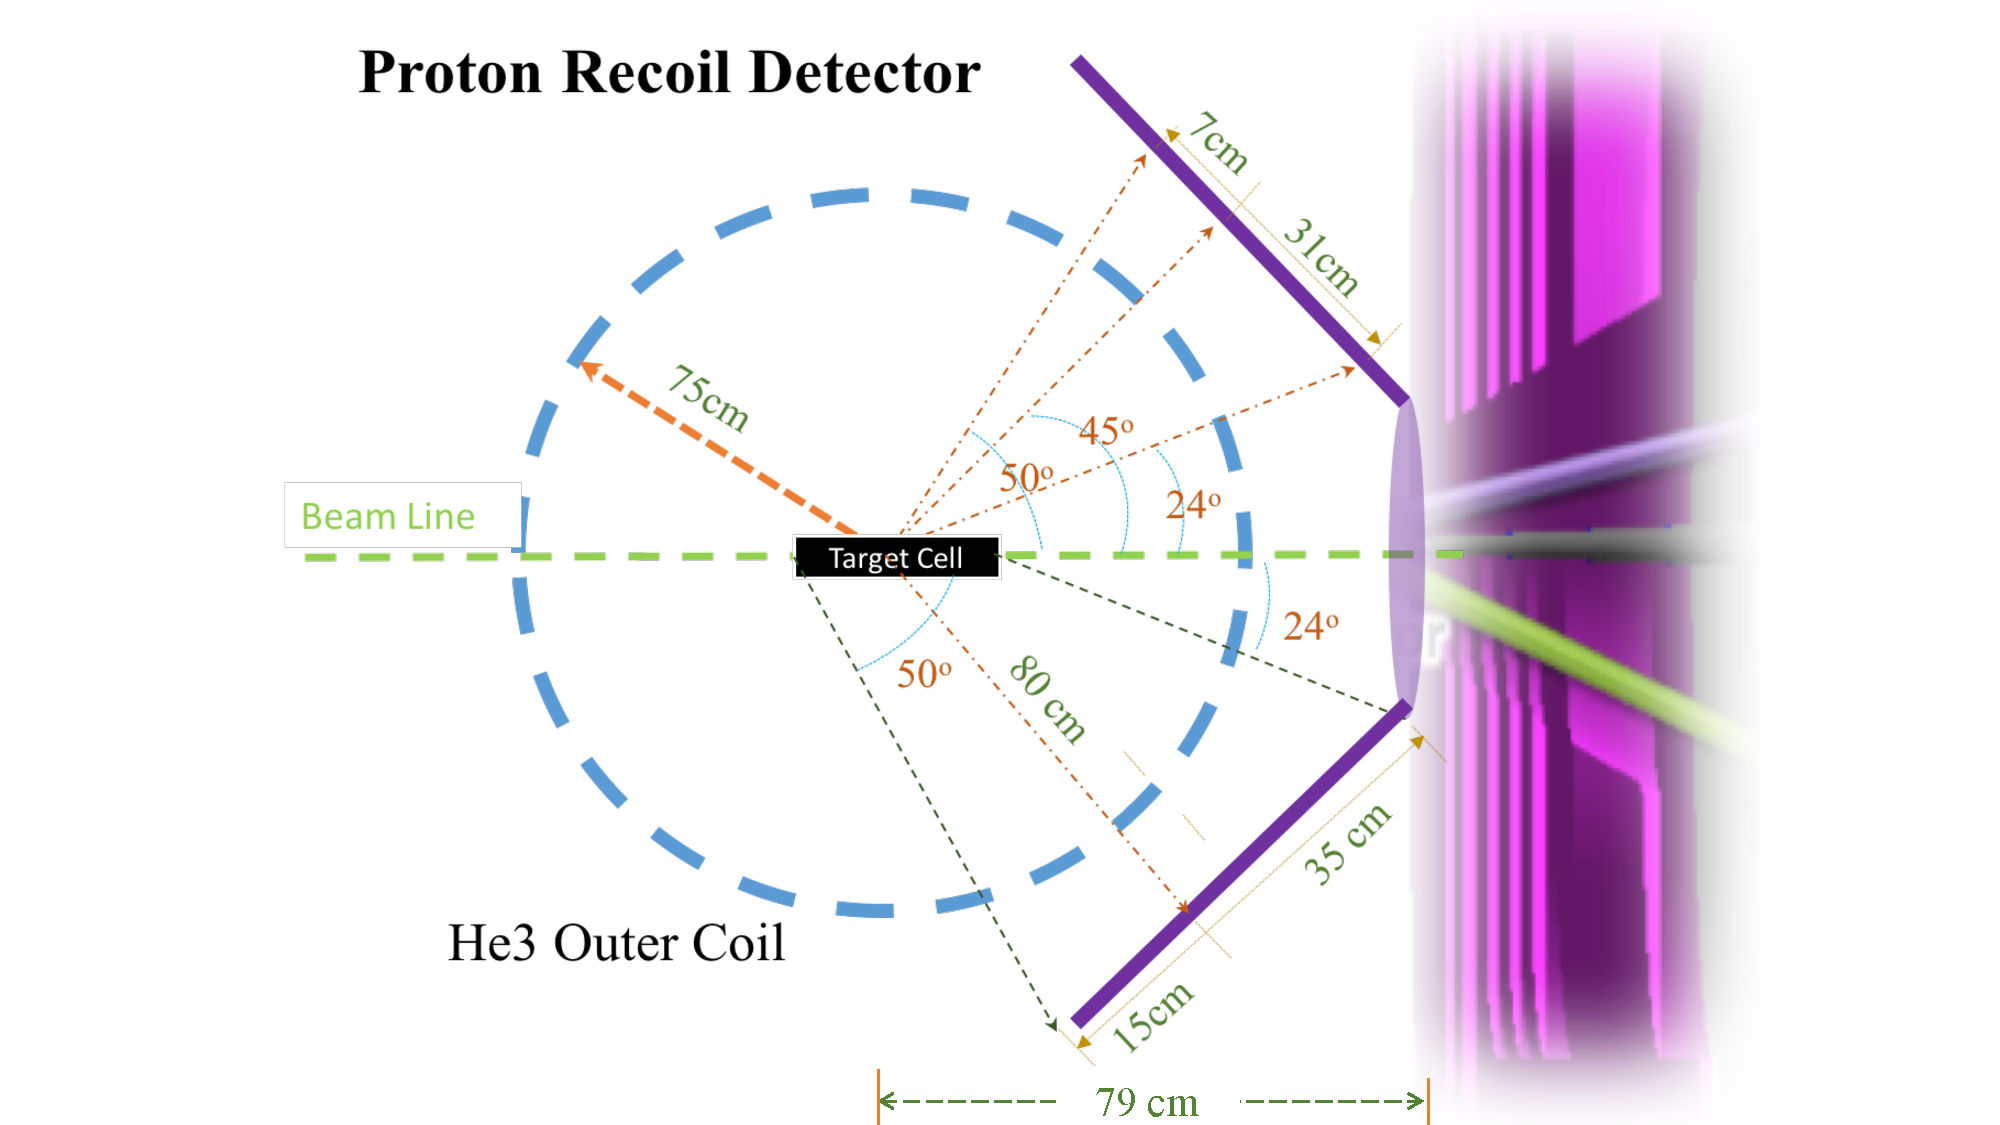
\includegraphics[width=0.7\textwidth]{./figures/prd_solid.pdf}
   \caption[Scheme of the new proton recoil detector ]{\footnotesize{Scheme of
       the new proton recoil detector. Such a cone-shape detector will be
       placed outside the outer Helmholtz coil of the $\mathrm{^{3}He}$ target
       system, covering polar angles from 24$^{\circ}$ to 50$^{\circ}$ and with
       2$\pi$ acceptance in azimuthal angle. We assume the detector plane
       to be tilted by -45$^{\circ}$ w.r.t. the beam direction with the
       vertical distance from the target center to the detector to be around
       80~cm. In this setting, the length of the detector is about 38~cm, and
       considering the target cell is 20~cm long, we extend the length to be
       50~cm. The inner and outer radius to be near 32~cm and 67~cm,
       respectively. The rough location of the solenoid is also indicated here. Note that lengths and locations are rough estimated, and the scales of angles and length are not proportional to the real scales.}}
   \label{prd_concept}
 \end{center}
\end{figure}
As shown in Fig.~\ref{prd_concept}, a new proton recoil detector (PRD) will be
placed right outside the $\mathrm{^{3}He}$ target system where the radius of
the outer Helmholtz coil is about 75~cm. The PRD will need to cover the polar
angle from 24$^{\circ}$ to 50$^{\circ}$ and provide full acceptance in
azimuthal angle. To minimize the detector area, the detector plane is tilted by
-45$^{\circ}$ along the beam direction and the vertical distance from the plane
to the target center is about 80~cm. After taking into account that the target
cell is 20~cm long, we require the length of the detector to be 50 cm, and its
inner and outer radii to be 32 cm and 67 cm, respectively.

To successfully select protons, we require the timing resolution of the
detector to be better than 60~ps, as discussed in Section 2.3. Since the
detector is close to the target and will suffer a huge background of low energy
particles, particularly low energy electrons, the detector will be divided
into fine segments to avoid pile-up of background signals. In addition, a thin
aluminum sheet of $\sim$4.5~mm thickness in front of the detector should be
able to block most of low energy particles. The rough angular information
provided by this detector will be helpful to further reject
background and isolate protons during the offline data analysis when
reconstructing missing mass and momentum.

\subsection{Scintillating Fiber Tracker}

One of the good candidates for the PRD is a scintillating fiber tracker
(SFT)~\cite{sft_zye}. Scintillating fibers (SciFi) have now been largely used
in experiments of particle physics because of its fast timing response and
flexibility, and several commercial manufacturers are able to produce high
quality fibers and at relatively low prices. Instead of using traditional large
paddles, we can construct the PRD by grouping SciFi in arrays and form the
detector planes.  With two planes of fibers at perpendicular directions, the
PRD can also provide position information by determining which fiber is fired
in each plane. A 1-mm round fiber is able to provide a 0.5~mm position
resolution and with a distance of 80~cm away from the target center, the
angular resolution can be better than 0.5~mrad, which can be essential to
further isolate protons and reduce background. On top of that, the SciFi is
highly segmented so the rate of random low energy background particles hitting
on a single fiber can be largely minimized, and the pile-up effect should be
significantly reduced compared with large area scintillator paddles.

We will choose silicon photo-multipliers (SiPM) as the photon-detectors to
collect light produced in the fibers. SiPM is idea for low-photon-number
counting since the light yield produced by a SciFi is not as strong as one
produced in a thin scintillator paddle. It is also not sensitive to magnetic
field, while the PRD will be placed in between the target system and the SoLID
magnet which both have strong magnetic field. Besides, there will be a lot of
read out channels and the price of SiPM is low enough to make the new detector
affordable.  The combination of SciFi and SiPM will make the PRD a very compact
detector which is very important since the space between the target system and
the solenoid magnet is limited.

A prototype project, funded by JSA postdoctoral fellow award \cite{sft_zye},
has been under development and we expect to build a small SFT and test its
performance near a target system with electron beam at JLab.

%\subsection{GEANT4 Simulation}

